% Architecture diagram - Context-Aware Alert Prioritization for Wazuh (Fig. 1)
%
% Standalone compile:   pdflatex architecture.tex
% Include in the paper: 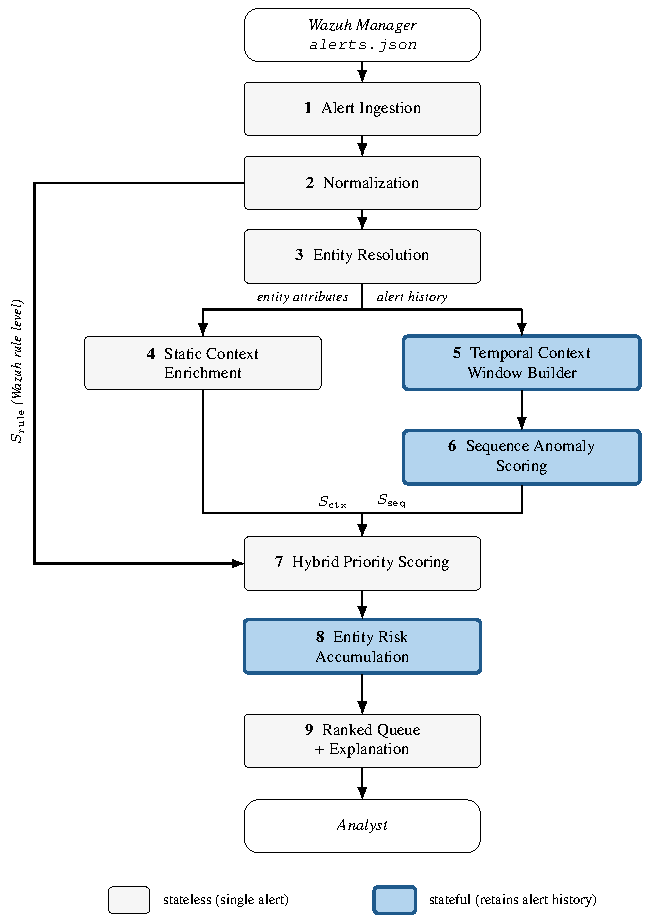
\includegraphics[width=\columnwidth]{architecture.pdf}
%
% Shading carries meaning: tinted boxes hold state across alerts, light boxes do not.
% Revision 3 (2026-10-11): Component 4 renamed (S_exp); Component 9 ranks repeat
% groups; admission filter named on Component 1.
\documentclass[border=4pt]{standalone}
\usepackage{times}
\usepackage{tikz}
\usepackage{xcolor}
\usetikzlibrary{arrows.meta,positioning}

\definecolor{statefulfill}{RGB}{179,212,238}
\definecolor{statefuledge}{RGB}{31,90,140}
\definecolor{statelessfill}{RGB}{246,246,246}

\begin{document}
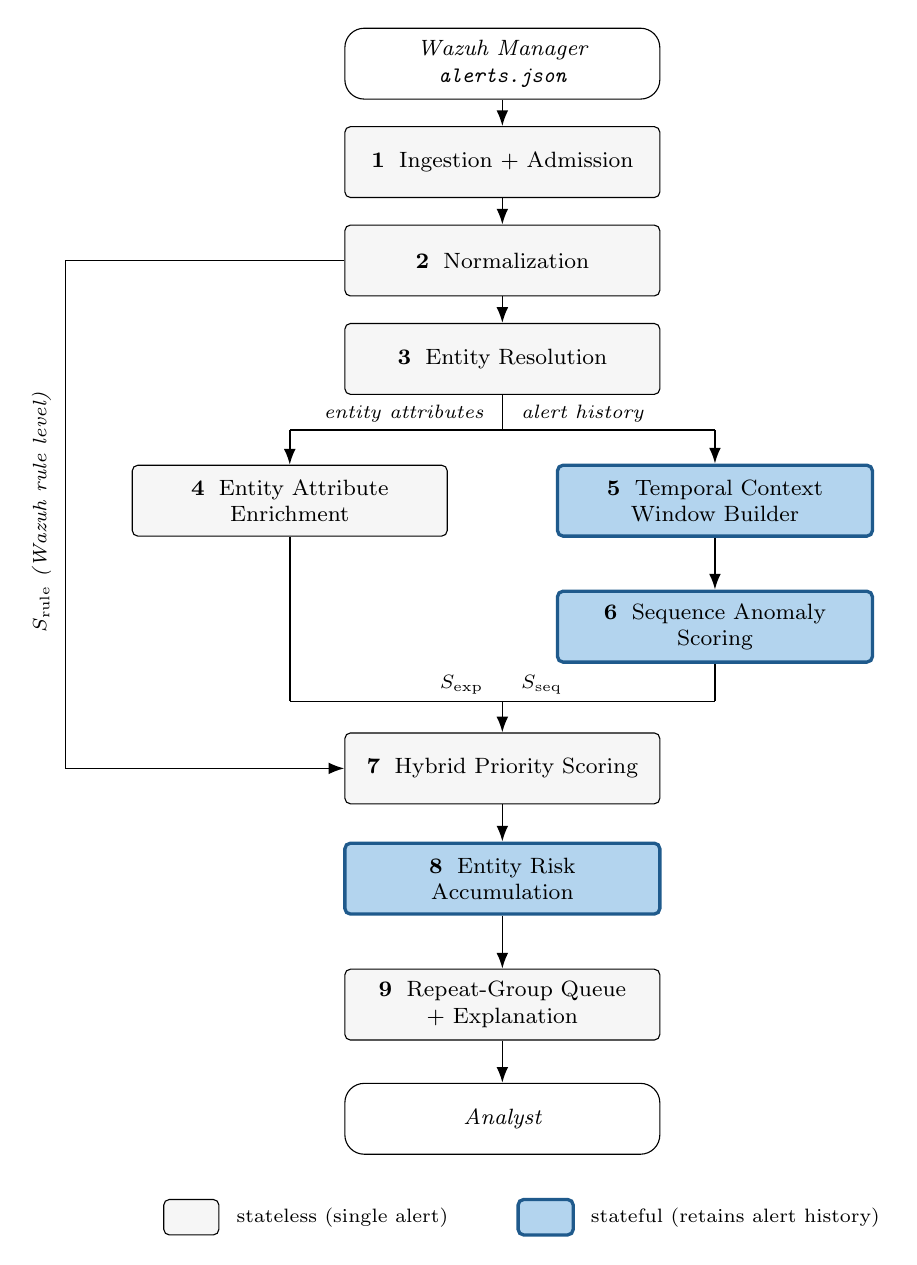
\begin{tikzpicture}[
  box/.style     = {draw, rounded corners=2pt, align=center, font=\footnotesize,
                    minimum height=9mm, minimum width=40mm, fill=statelessfill},
  stateful/.style= {box, fill=statefulfill, draw=statefuledge, very thick},
  term/.style    = {draw, rounded corners=7pt, align=center, font=\footnotesize\itshape,
                    minimum height=9mm, minimum width=40mm, fill=white},
  fl/.style      = {-{Latex[length=2mm]}, semithick},
  ln/.style      = {semithick},
  tag/.style     = {font=\scriptsize\itshape, inner sep=1.5pt}
]

\node[term]     at (0,0)       (wazuh) {Wazuh Manager\\\texttt{alerts.json}};
\node[box]      at (0,-1.25)   (c1) {\textbf{1}\; Ingestion + Admission};
\node[box]      at (0,-2.50)   (c2) {\textbf{2}\; Normalization};
\node[box]      at (0,-3.75)   (c3) {\textbf{3}\; Entity Resolution};

\node[box]      at (-2.7,-5.55) (c4) {\textbf{4}\; Entity Attribute\\Enrichment};
\node[stateful] at ( 2.7,-5.55) (c5) {\textbf{5}\; Temporal Context\\Window Builder};
\node[stateful] at ( 2.7,-7.15) (c6) {\textbf{6}\; Sequence Anomaly\\Scoring};

\node[box]      at (0,-8.95)   (c7) {\textbf{7}\; Hybrid Priority Scoring};
\node[stateful] at (0,-10.35)  (c8) {\textbf{8}\; Entity Risk\\Accumulation};
\node[box]      at (0,-11.95)  (c9) {\textbf{9}\; Repeat-Group Queue\\ + Explanation};
\node[term]     at (0,-13.40)  (an) {Analyst};

\draw[fl] (wazuh) -- (c1);
\draw[fl] (c1) -- (c2);
\draw[fl] (c2) -- (c3);

\draw[ln] (c3.south) -- (0,-4.65);
\draw[ln] (-2.7,-4.65) -- (2.7,-4.65);
\draw[fl] (-2.7,-4.65) -- (c4.north);
\draw[fl] ( 2.7,-4.65) -- (c5.north);
\node[tag, anchor=south east] at (-0.18,-4.62) {entity attributes};
\node[tag, anchor=south west] at ( 0.18,-4.62) {alert history};

\draw[fl] (c5) -- (c6);

\draw[ln] (c4.south) -- (-2.7,-8.10);
\draw[ln] (c6.south) -- ( 2.7,-8.10);
\draw[ln] (-2.7,-8.10) -- (2.7,-8.10);
\draw[fl] (0,-8.10) -- (c7.north);
\node[tag, anchor=south east] at (-0.18,-8.07) {$S_\mathrm{exp}$};
\node[tag, anchor=south west] at ( 0.18,-8.07) {$S_\mathrm{seq}$};

\draw[ln] (c2.west) -- (-5.55,-2.50);
\draw[fl] (-5.55,-2.50) -- (-5.55,-8.95) -- (c7.west);
\node[tag, rotate=90, anchor=south] at (-5.67,-5.7) {$S_\mathrm{rule}$ (Wazuh rule level)};

\draw[fl] (c7) -- (c8);
\draw[fl] (c8) -- (c9);
\draw[fl] (c9) -- (an);

\node[box, minimum width=7mm, minimum height=4.5mm] at (-3.95,-14.65) (lg1) {};
\node[anchor=west, font=\scriptsize] at (-3.50,-14.65) {stateless (single alert)};
\node[stateful, minimum width=7mm, minimum height=4.5mm] at (0.55,-14.65) (lg2) {};
\node[anchor=west, font=\scriptsize] at (1.00,-14.65) {stateful (retains alert history)};

\end{tikzpicture}
\end{document}
